\definecolor{grey_blue}{RGB}{195,90,125}
\definecolor{dark_red}{RGB}{77,16,16}

\pgfplotsset{%
    ,compat=1.12
    ,every axis x label/.style={at={(current axis.right of origin)},anchor=north west}
    ,every axis y label/.style={at={(current axis.above origin)},anchor=north east}
    }

\scalebox{0.9}{ %%% scale it
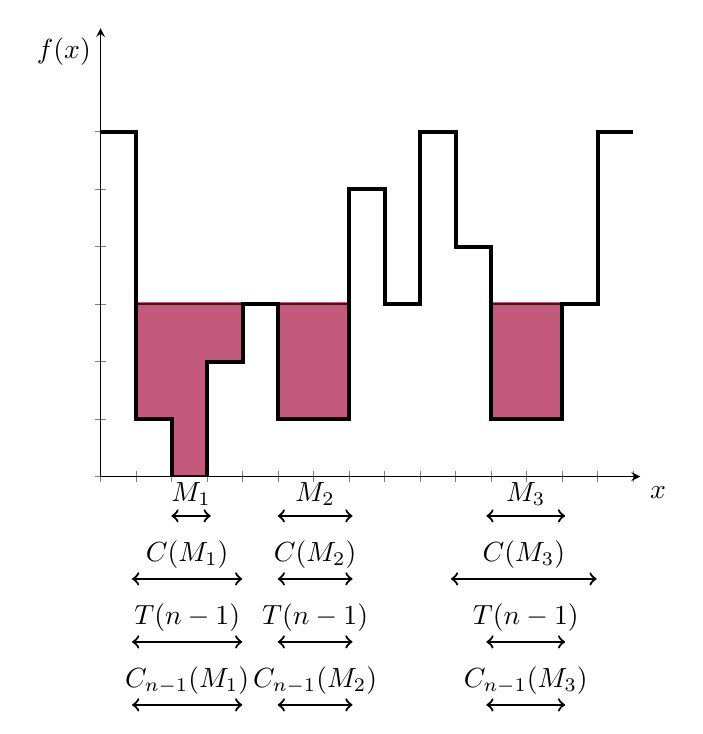
\begin{tikzpicture}

\tikzset{
    arr_black/.style={<->,black,thick},
    shadowed/.style={preaction={transform canvas={shift={(0pt,-1pt)}},draw=gray,very thick}},
    shadowed_blue/.style={preaction={transform canvas={shift={(0pt,-3.5pt)}},draw=grey_blue,very thick,line width=3mm}},
  }
\begin{axis}[%
    ,xlabel=$x$
    ,ylabel=$f(x)$
    ,axis x line = bottom,axis y line = left
    ,ytick={0.0,0.25,...,1.75}
    ,xtick={0.0,0.25,...,3.75}
    ,ymax=2.2 % or enlarge y limits=upper
    ,xmax=3.8
    ,yticklabels={,,}
    ,xticklabels={,,}
    ]
% water: 1.0 -> 1.25
%%%%%%%%%%%%%%
%CB1
\addplot+[const plot, no marks, thick, dark_red, line width=.3mm, shadowed_blue] coordinates { (0.25, 1) (1, 1)} node[above,pos=.57,black] {$ $};
\addplot+[const plot, no marks, thick, grey_blue, line width=14mm, shadowed_blue] coordinates { (0.26, .75) (.51, .75)} node[below,pos=.57,black] {$ $};

\addplot+[const plot, no marks, thick, grey_blue, line width=40mm, shadowed_blue] coordinates { (0.5, 0.25) (.75, 0.25)} node[below,pos=.57,black] {$ $};

\addplot+[const plot, no marks, thick, grey_blue, line width=6mm, shadowed_blue] coordinates { (0.74, 0.85) (1, 0.85)} node[below,pos=.57,black] {$ $};
%%%%%%%%%%%%%%
%CB2
\addplot+[const plot, no marks, thick, dark_red, line width=.3mm, shadowed_blue] coordinates { (1.25, 1) (1.75, 1)} node[above,pos=.57,black] {$ $};

\addplot+[const plot, no marks, solid, thick, grey_blue, line width=13.5mm, shadowed_blue] coordinates { (1.25, .74) (1.75, .74)} node[above,pos=.57,black] {$ $};

%%%%%%%%%%%%%
%CB3
\addplot+[const plot, no marks, solid, thick, dark_red, line width=.3mm, shadowed_blue] coordinates { (2.75, 1) (3.25, 1)} node[above,pos=.57,black] {$ $};

\addplot+[const plot, no marks, solid, thick, grey_blue, line width=13mm, shadowed_blue] coordinates { (2.75, .725) (3.25, .725)} node[above,pos=.57,black] {$ $};


%%%%%%%%%%%%%%%%%
% graph
\addplot+[const plot, no marks, thick, solid, black, line width=.5mm] coordinates {(0,1.75) (0.25,1.75) (0.25,0.5) (0.5,0.5) (0.5,0.25) (0.75,0.75) (1,1) (1.25, 0.5) (1.75,1.5) (2, 1.0) (2.25, 1.75) (2.5, 1.25) (2.75, 0.5) (3.25, 1.0) (3.5, 1.75) (3.75, 1.75)} node[above,pos=.57,black] {$ $};


\end{axis}

% minima
\draw [arr_black] (0.9,-0.5) --node [above]{$M_1$} (1.4,-0.5);
\draw [arr_black] (2.25,-0.5) --node [above]{$M_2$} (3.2,-0.5);
\draw [arr_black] (4.9,-0.5) --node [above]{$M_3$} (5.9,-0.5);

% catchment  basins
\draw [arr_black] (0.4,-1.3) --node [above]{$C(M_1)$} (1.8,-1.3);
\draw [arr_black] (2.25,-1.3) --node [above]{$C(M_2)$} (3.2,-1.3);
\draw [arr_black] (4.45,-1.3) --node [above]{$C(M_3)$} (6.3,-1.3);

% threshold
\draw [arr_black] (0.4,-2.1) --node [above]{$T(n-1)$} (1.8,-2.1);
\draw [arr_black] (2.25,-2.1) --node [above]{$T(n-1)$} (3.2,-2.1);
\draw [arr_black] (4.9,-2.1) --node [above]{$T(n-1)$} (5.9,-2.1);

% Cn(Mi)
\draw [arr_black] (0.4,-2.9) --node [above]{$C_{n-1}(M_1)$} (1.8,-2.9);
\draw [arr_black] (2.25,-2.9) --node [above]{$C_{n-1}(M_2)$} (3.2,-2.9);
\draw [arr_black] (4.9,-2.9) --node [above]{$C_{n-1}(M_3)$} (5.9,-2.9);


\end{tikzpicture}
} %%% finish scaling
